\begin{table}[htbp]
 \centering
 \caption{The result of the user study (line)}
 \begin{tabular}{lccc}
\toprule
 & Trial 1 & Trial 2 & Trial 3\\
\midrule
 User A (VI)&
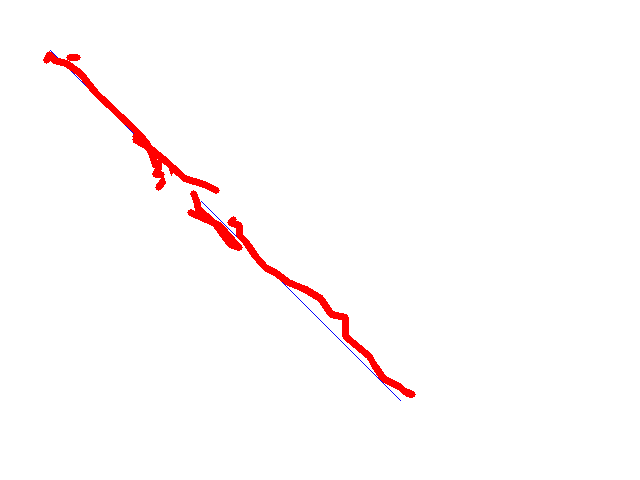
\includegraphics[width=3cm]{fig_exp/line_Ayaka_test3_0.png} &
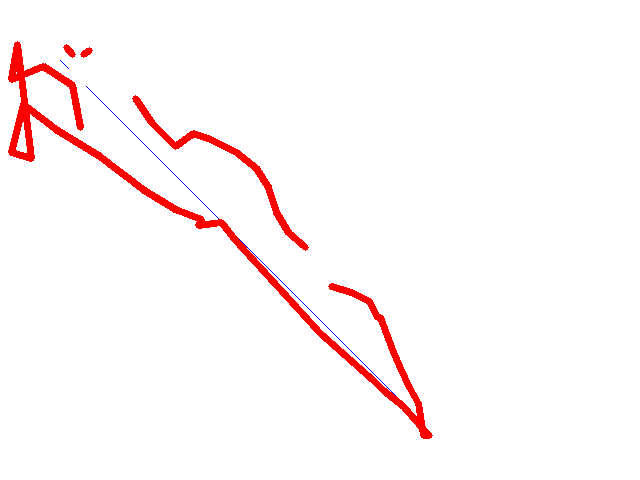
\includegraphics[width=3cm]{fig_exp/line_Ayaka_test3_1.png} &
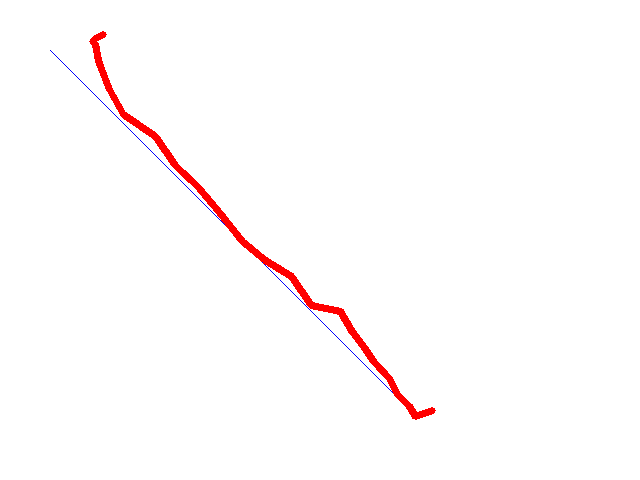
\includegraphics[width=3cm]{fig_exp/line_Ayaka_test3_2.png} \\
\midrule
 User B (VI)&
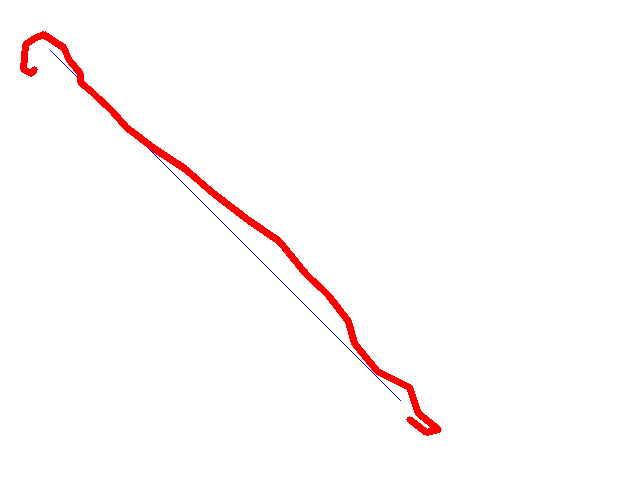
\includegraphics[width=3cm]{fig_exp/line_Angus_test3_0.png} &
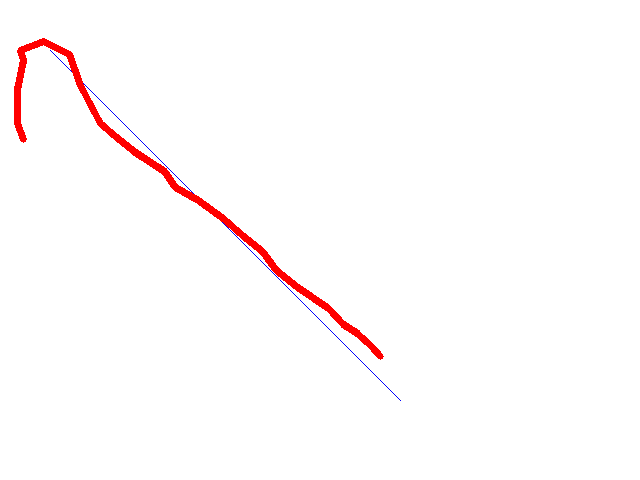
\includegraphics[width=3cm]{fig_exp/line_Angus_test3_1.png} &
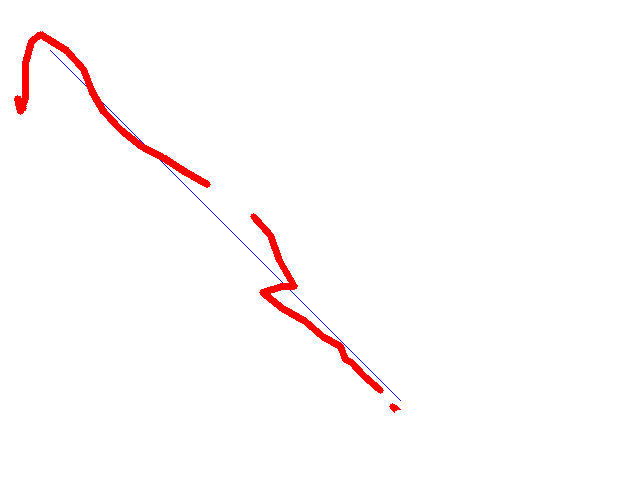
\includegraphics[width=3cm]{fig_exp/line_Angus_test3_2.png} \\
\midrule
 User A (Mouse)&
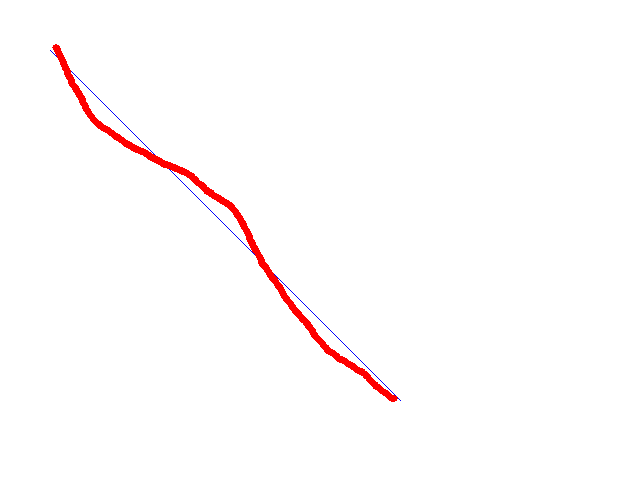
\includegraphics[width=3cm]{fig_exp/line_Ayaka_test3_0_m.png} &
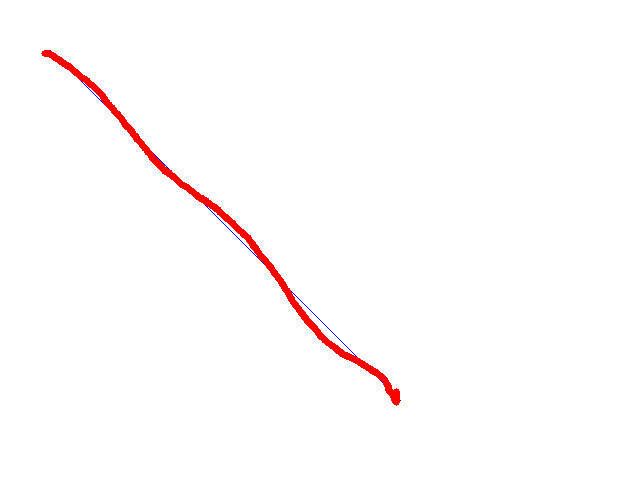
\includegraphics[width=3cm]{fig_exp/line_Ayaka_test3_1_m.png} &
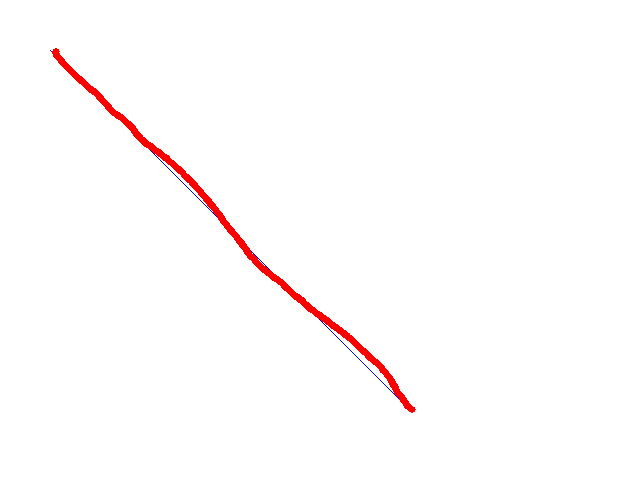
\includegraphics[width=3cm]{fig_exp/line_Ayaka_test3_2_m.png} \\
\midrule
 User B (Mouse)&
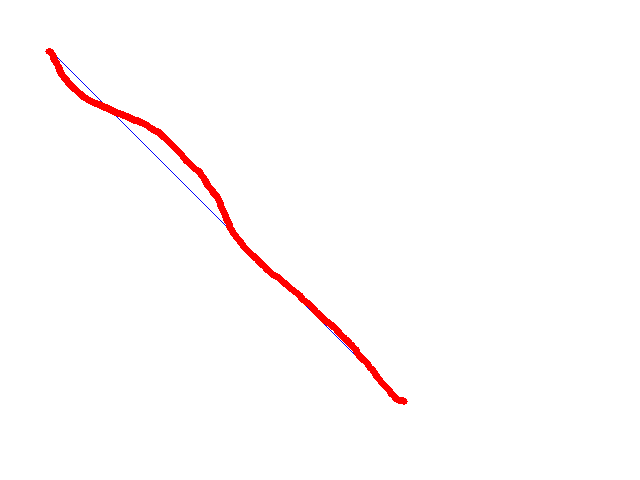
\includegraphics[width=3cm]{fig_exp/line_Angus_test3_0_m.png} &
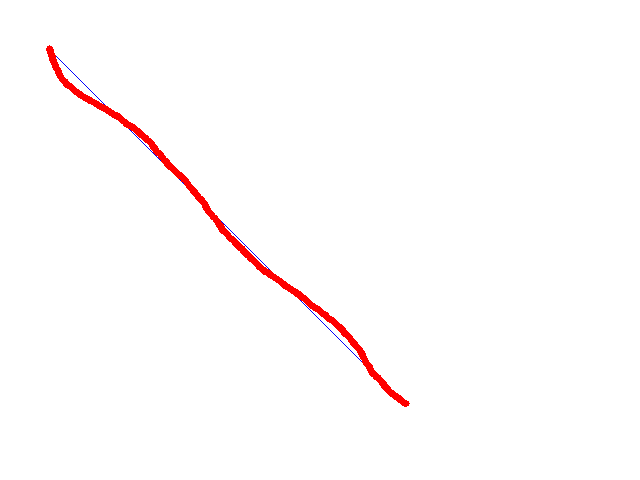
\includegraphics[width=3cm]{fig_exp/line_Angus_test3_1_m.png} &
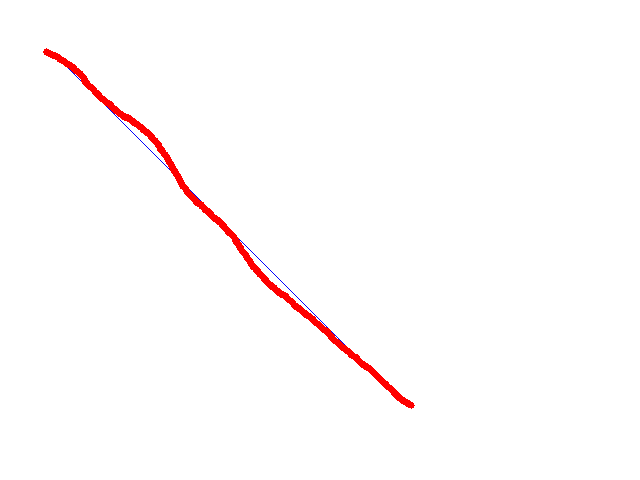
\includegraphics[width=3cm]{fig_exp/line_Angus_test3_2_m.png} \\
\bottomrule
\end{tabular}

\end{table}
\begin{table}[htbp]
 \centering
 \caption{The result of the user study (circle)}
 \begin{tabular}{lccc}
\toprule
 & Trial 1 & Trial 2 & Trial 3\\
\midrule
 User A (VI)&
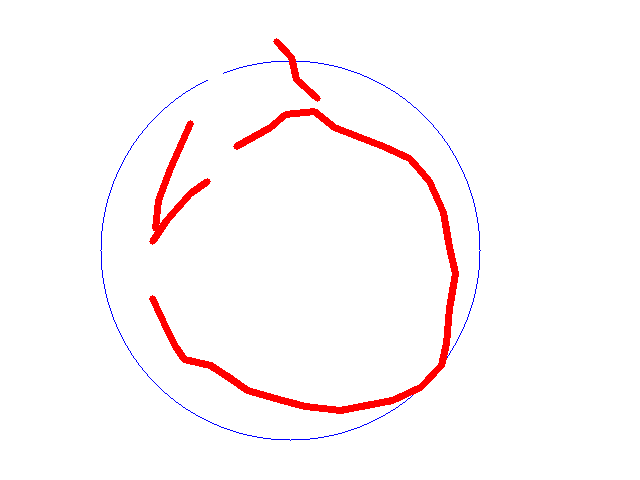
\includegraphics[width=3cm]{fig_exp/circle_Ayaka_test3_0.png} &
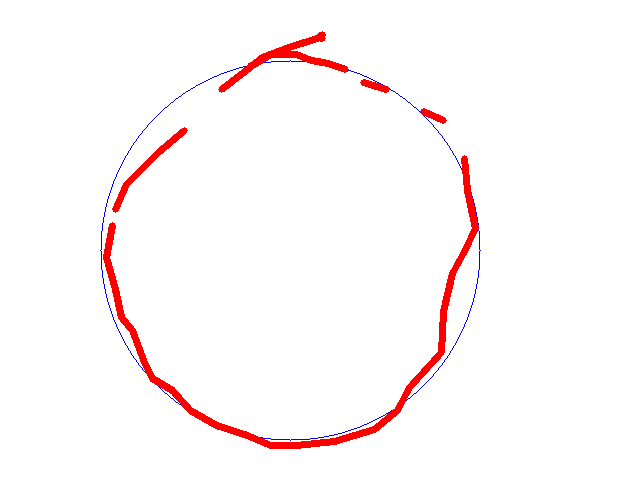
\includegraphics[width=3cm]{fig_exp/circle_Ayaka_test3_1.png} &
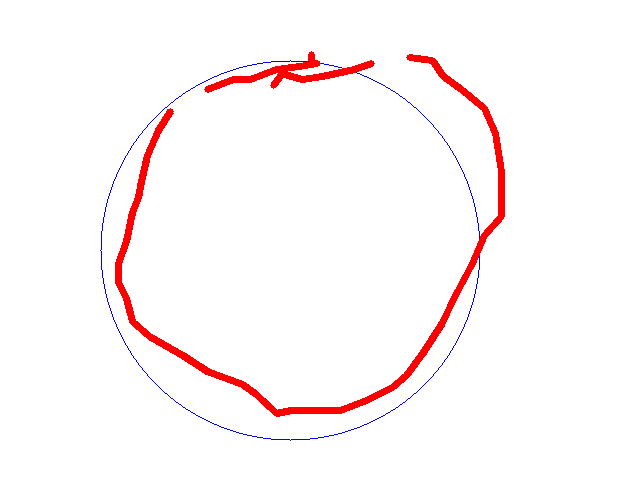
\includegraphics[width=3cm]{fig_exp/circle_Ayaka_test3_2.png} \\
\midrule
 User B (VI)&
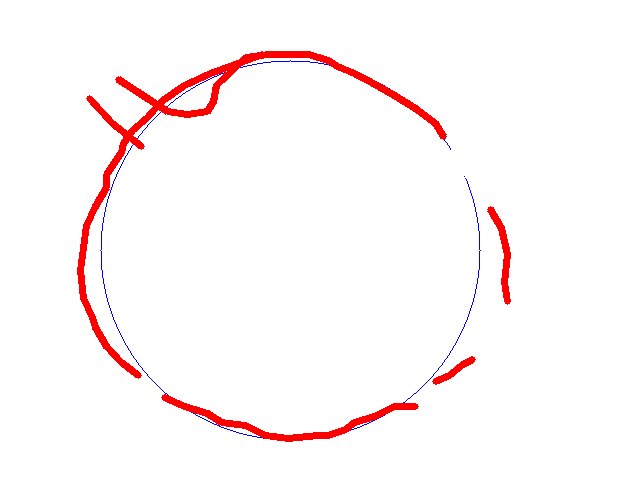
\includegraphics[width=3cm]{fig_exp/circle_Angus_test3_0.png} &
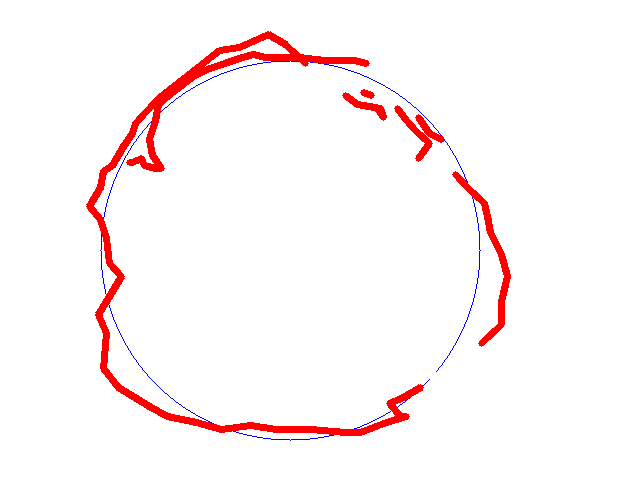
\includegraphics[width=3cm]{fig_exp/circle_Angus_test3_1.png} &
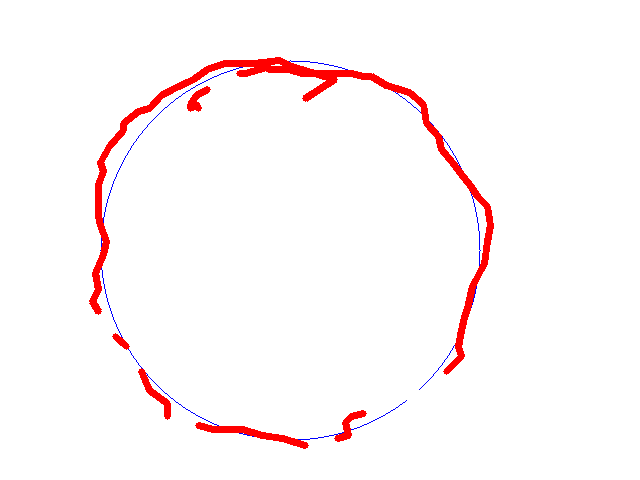
\includegraphics[width=3cm]{fig_exp/circle_Angus_test3_2.png} \\
\midrule
 User A (Mouse)&
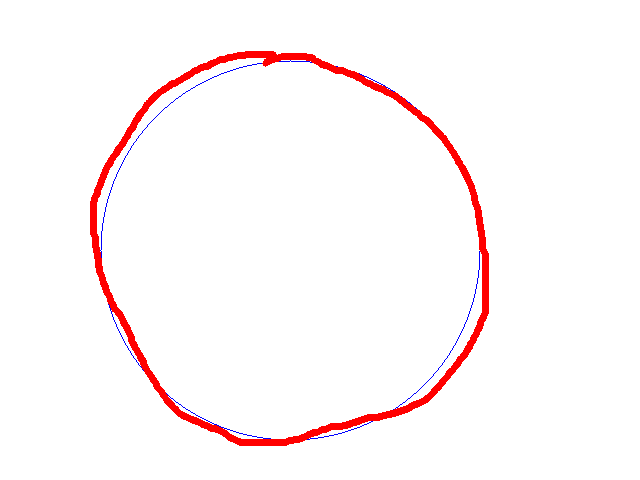
\includegraphics[width=3cm]{fig_exp/circle_Ayaka_test3_0_m.png} &
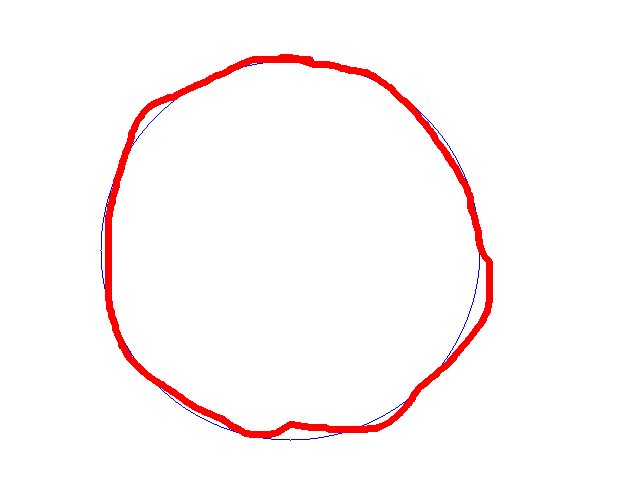
\includegraphics[width=3cm]{fig_exp/circle_Ayaka_test3_1_m.png} &
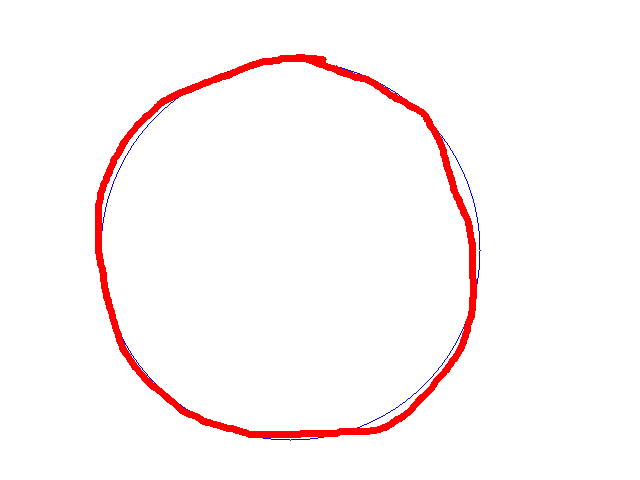
\includegraphics[width=3cm]{fig_exp/circle_Ayaka_test3_2_m.png} \\
\midrule
 User B (Mouse)&
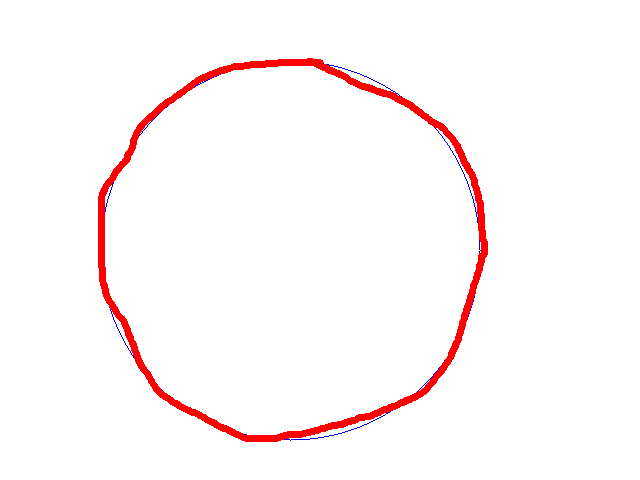
\includegraphics[width=3cm]{fig_exp/circle_Angus_test3_0_m.png} &
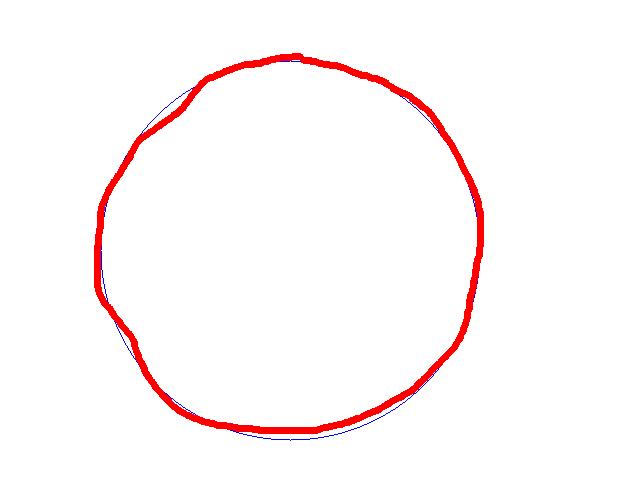
\includegraphics[width=3cm]{fig_exp/circle_Angus_test3_1_m.png} &
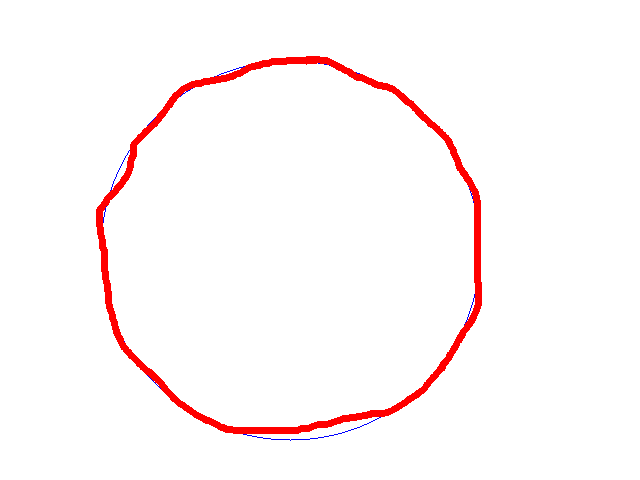
\includegraphics[width=3cm]{fig_exp/circle_Angus_test3_2_m.png} \\
\bottomrule
\end{tabular}


\end{table}

\begin{table}[htbp]
 \centering
 \caption{The result of the user study (line)}
 \begin{tabular}{llrrr}
 \toprule
 User & Device & Trial & Time[sec] & Error Pixels \\
 \midrule
 A	& VI	  & 1	& 20.16	& 22.25 \\
 A	& VI	  & 2	& 14.75	& 76.46 \\
 A	& VI	  & 3	& 5.73	& 25.77 \\
 B	& VI	  & 1	& 7.76	& 39.92 \\
 B	& VI	  & 2	& 8.03	& 88.50 \\
 B	& VI	  & 3	& 10.03	& 58.27 \\
 A	& Mouse	& 1	& 4.07	& 13.87 \\
 A	& Mouse	& 2	& 5.19	& 6.53 \\
 A	& Mouse	& 3	& 4.07	& 8.01 \\
 B	& Mouse	& 1	& 3.98	& 8.99 \\
 B	& Mouse	& 2	& 4.83	& 7.24 \\
 B	& Mouse	& 3	& 4.61	& 7.71 \\
 \bottomrule
\end{tabular}

\end{table}
\begin{table}[htbp]
 \centering
 \caption{The result of the user study (line)}
 \begin{tabular}{llrrr}
 \toprule
 User & Device & Trial & Time[sec] & Error [pixels] \\
 \midrule
A	&	VI	&	1	&	14.507	&	12.745	\\
A	&	VI	&	2	&	17.756	&	18.283	\\
A	&	VI	&	3	&	20.314	&	17.653	\\
B	&	VI	&	1	&	8.131	&	24.242	\\
B	&	VI	&	2	&	7.84	&	14.619	\\
B	&	VI	&	3	&	7.962	&	13.559	\\
C	&	VI	&	1	&	8.433	&	46.652	\\
C	&	VI	&	2	&	10.818	&	17.856	\\
C	&	VI	&	3	&	11.376	&	10.398	\\
A	&	VI2	&	1	&	20.229	&	6.966	\\
A	&	VI2	&	2	&	17.148	&	9.991	\\
A	&	VI2	&	3	&	17.836	&	7.156	\\
B	&	VI2	&	1	&	10.819	&	12.892	\\
B	&	VI2	&	2	&	11.19	&	13.977	\\
B	&	VI2	&	3	&	12.79	&	17.879	\\
C	&	VI2	&	1	&	10.963	&	12.154	\\
C	&	VI2	&	2	&	11.597	&	7.066	\\
C	&	VI2	&	3	&	12.712	&	8.156	\\
A	&	Mouse	&	1	&	8.187	&	8.815	\\
A	&	Mouse	&	2	&	10.502	&	4.736	\\
A	&	Mouse	&	3	&	9.929	&	5.995	\\
B	&	Mouse	&	1	&	8.801	&	4.548	\\
B	&	Mouse	&	2	&	7.999	&	4.067	\\
B	&	Mouse	&	3	&	8.039	&	4.741	\\
C	&	Mouse	&	1	&	7.474	&	6.215	\\
C	&	Mouse	&	2	&	7.187	&	6.929	\\
C	&	Mouse	&	3	&	7.519	&	5.348	\\
 \bottomrule
\end{tabular}

\end{table}
\begin{table}[htbp]
 \centering
 \caption{The result of the user study (line)}
 \begin{tabular}{llrrr}
 \toprule
 User & Device & Trial & Time[sec] & Error [pixels] \\
 \midrule
A	&	VI	&	1	&	13.32	&	68.558	\\
A	&	VI	&	2	&	14.522	&	88.314	\\
A	&	VI	&	3	&	15.282	&	68.406	\\
B	&	VI	&	1	&	17.87	&	72.838	\\
B	&	VI	&	2	&	12.132	&	68.172	\\
B	&	VI	&	3	&	6.599	&	71.913	\\
C	&	VI	&	1	&	13.127	&	74.432	\\
C	&	VI	&	2	&	14.004	&	51.564	\\
C	&	VI	&	3	&	13.183	&	67.076	\\
A	&	VI2	&	1	&	11.856	&	63.8	\\
A	&	VI2	&	2	&	12.086	&	58.081	\\
A	&	VI2	&	3	&	18.693	&	89.614	\\
B	&	VI2	&	1	&	10.93	&	88.821	\\
B	&	VI2	&	2	&	13.809	&	104.269	\\
B	&	VI2	&	3	&	8.009	&	67.539	\\
C	&	VI2	&	1	&	18.943	&	31.226	\\
C	&	VI2	&	2	&	17.128	&	66.85	\\
C	&	VI2	&	3	&	16.892	&	87.412	\\
A	&	Mouse	&	1	&	6.716	&	4.125	\\
A	&	Mouse	&	2	&	7.444	&	10.296	\\
A	&	Mouse	&	3	&	7	&	4.634	\\
B	&	Mouse	&	1	&	8.113	&	4.746	\\
B	&	Mouse	&	2	&	6.293	&	8.115	\\
B	&	Mouse	&	3	&	6.428	&	7.388	\\
C	&	Mouse	&	1	&	5.4	&	4.989	\\
C	&	Mouse	&	2	&	5.481	&	4.768	\\
C	&	Mouse	&	3	&	5.199	&	6.603	\\
 \bottomrule
\end{tabular}

\end{table}
\begin{table}[htbp]
 \centering
 \caption{Standard Deviation of User study}
 \begin{tabular}{lllrr}
 \toprule
 Task & User & Device & StdDev of Time & StdDev of Error \\
 \midrule
 Points	& A	& VI	  & 2.20	& 9.87 \\
 Points	& B	& VI	  & 1.37	& 10.06 \\
 Points	& A	& Mouse	& 0.83	& 1.29 \\
 Points	& B	& Mouse	& 0.46	& 0.31 \\
 Circle	& A	& VI	  & 0.28	& 11.75 \\
 Circle	& B	& VI	  & 1.88	& 2.23 \\
 Circle	& A	& Mouse	& 0.07	& 0.80 \\
 Circle	& B	& Mouse	& 0.25	& 0.26 \\
 Line	  & A	& VI	  & 5.95	& 24.77 \\
 Line	  & B	& VI	  & 1.01	& 20.03 \\
 Line	  & A	& Mouse	& 0.53	& 3.17 \\
 Line	  & B	& Mouse	& 0.36	& 0.74 \\
 \bottomrule
\end{tabular}

\end{table}

\begin{figure}
 \centering
 \begin{tikzpicture}
\node[anchor=north west,inner sep=0] (image) at (0,0) {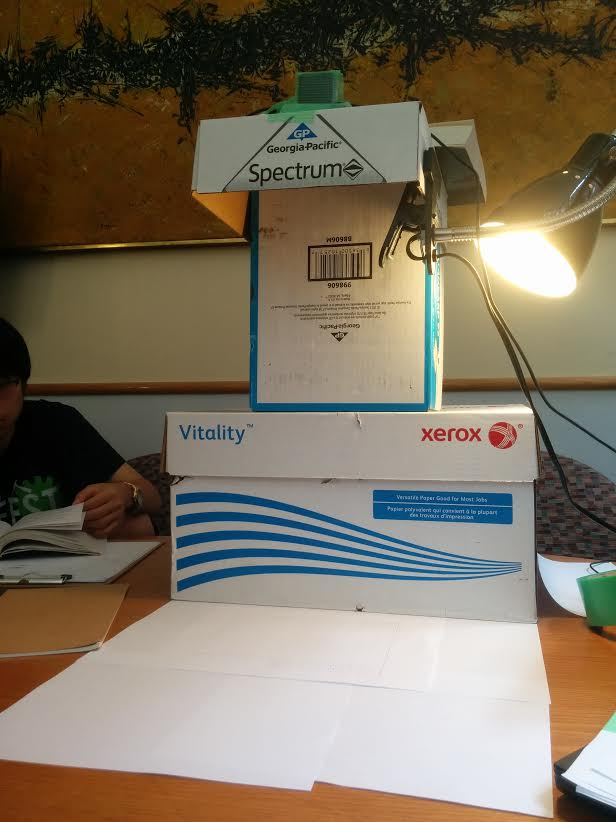
\includegraphics[width=7cm]{device.jpg}};
\begin{scope}[x={7cm / 616},y={-7cm / 616}]
 \draw[red,ultra thick,<-] (350, 90) -- ++(50, 0) node[right,font=\bf\Large] {Camera};
 \draw[red,ultra thick,<-] (520, 320) -- ++(-50, 50) node[below,font=\bf\Large] {Light source};
 \draw[red,ultra thick,<-] (340, 720) node[below,font=\bf\Large] {Paper canvas};
\end{scope}
\end{tikzpicture}

 \caption{The input device}
\end{figure}
